\documentclass[journal]{IEEEtran}

  \usepackage{graphicx}
  \usepackage{fixltx2e}
  \usepackage{stfloats}
  \usepackage{listings}

  \usepackage{tikz}
  \usetikzlibrary{shapes.multipart}  
  
  \usepackage{pgfplots}


\pgfplotsset{
    box plot/.style={
        /pgfplots/.cd,
        black,
        only marks,
        mark=-,
        mark size=0.2em,
        /pgfplots/error bars/.cd,
        y dir=plus,
        y explicit,
    },
    box plot box/.style={
        /pgfplots/error bars/draw error bar/.code 2 args={%
            \draw  ##1 -- ++(0.2em,0pt) |- ##2 -- ++(-0.2em,0pt) |- ##1 -- cycle;
        },
        /pgfplots/table/.cd,
        y index=2,
        y error expr={\thisrowno{3}-\thisrowno{2}},
        /pgfplots/box plot
    },
    box plot top whisker/.style={
        /pgfplots/error bars/draw error bar/.code 2 args={%
            \pgfkeysgetvalue{/pgfplots/error bars/error mark}%
            {\pgfplotserrorbarsmark}%
            \pgfkeysgetvalue{/pgfplots/error bars/error mark options}%
            {\pgfplotserrorbarsmarkopts}%
            \path ##1 -- ##2;
        },
        /pgfplots/table/.cd,
        y index=4,
        y error expr={\thisrowno{2}-\thisrowno{4}},
        /pgfplots/box plot,
    },
    box plot bottom whisker/.style={
        /pgfplots/error bars/draw error bar/.code 2 args={%
            \pgfkeysgetvalue{/pgfplots/error bars/error mark}%
            {\pgfplotserrorbarsmark}%
            \pgfkeysgetvalue{/pgfplots/error bars/error mark options}%
            {\pgfplotserrorbarsmarkopts}%
            \path ##1 -- ##2;
        },
        /pgfplots/table/.cd,
        y index=5,
        y error expr={\thisrowno{3}-\thisrowno{5}},
        /pgfplots/box plot
    },
    box plot median/.style={
        /pgfplots/box plot
    }
}

  

\begin{document}

\title{Project report}

\author{Vincent B\textsc{rillault} \& Pierre P\textsc{fister}}% <-this % stops a space


\markboth{Advanced Computer Networks and Distributed Systems 2012}%
{Shell \MakeLowercase{\textit{et al.}}: Bare Demo of IEEEtran.cls for Journals}
\maketitle





\begin{abstract}
\boldmath
%The abstract goes here.
\end{abstract}
%% IEEEtran.cls defaults to using nonbold math in the Abstract.
%% This preserves the distinction between vectors and scalars. However,
%% if the journal you are submitting to favors bold math in the abstract,
%% then you can use LaTeX's standard command \boldmath at the very start
%% of the abstract to achieve this. Many IEEE journals frown on math
%% in the abstract anyway.
%
%% Note that keywords are not normally used for peerreview papers.
%\begin{IEEEkeywords}
%IEEEtran, journal, \LaTeX, paper, template.
%\end{IEEEkeywords}






\section{Introduction}

\IEEEPARstart{C}{loud} computing and virtualization have become, in computer science, one of the hottest topic of the last few years.
Indeed, virtualization has been unanimously recognized as an elegant, flexible and effective way to distribute and isolate services in a very dynamic manner, which gracefully tolerate hardware failure.
Nevertheless, cloud computing is a matter of trade-off between performance and simplicity.
As a result, in order to be competitive, works have been done to enhance virtualization performances, and hyper-virtualization is one of the best solution.
Individual computing capacity of virtual machines do not suffer performance issue anymore, but, in the case of distributed systems, there is still room for optimization in the network stack.
Our project consists in creating an optimized exchange channel between two virtual machines running on a single Xen hypervisor which would improve both bandwidth and delays.

\subsection{Motivations}

Between normal virtual host, the standard communication channels use the network stack.
Between two applications, a message passing through the network stack will need to go into the local IP stack, travel from the host to dom0 through the virtual interface, be routed or switched back to the other host through the other virtual interface, follow the local IP stack and then arrive in the application.
Going through all those different parts results in successive copies of the same packet in different memories, thus cost a lot.
Furthermore as network interface use interruptions to indicate new packets, going through the network stack generate a lot of kernel context switch.

\begin{figure}[h]
  \centering
  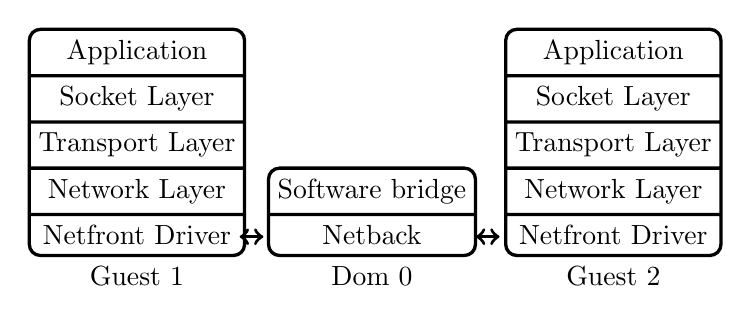
\begin{tikzpicture}
      [domU/.style={
           rectangle split,
           rectangle split parts=5,
           rounded corners,
           draw=black, very thick,
           text centered,
           anchor=five
         },
       dom0/.style={
           rectangle split,
           rectangle split parts=2,
           rounded corners,
           draw=black, very thick,
           text centered,
           anchor=two
         },
       ]
    \node [domU, label=below:Guest 1] (dom1) at (-3,0) {
      Application
      \nodepart{two}
      Socket Layer
      \nodepart{three}
      Transport Layer
      \nodepart{four}
      Network Layer
      \nodepart{five}
      Netfront Driver
    };
    
    \node [domU, label=below:Guest 2] (dom2) at (3.05,0) {
      Application
      \nodepart{two}
      Socket Layer
      \nodepart{three}
      Transport Layer
      \nodepart{four}
      Network Layer
      \nodepart{five}
      Netfront Driver
    };

    \node [dom0, label=below:Dom 0] (dom0) at (0.55,0) {
      Software bridge
      \nodepart{two}
      Netback
    };

    \path (-0.5,0.1) edge [draw=black, very thick, <->] (-0.2,0.1);
    \path (2.5,0.1) edge [draw=black, very thick, <->] (2.8,0.1);
    
  \end{tikzpicture}
  \caption{Normal IP architecture of Xen domUs}
  \label{xen_normal_architecture}
\end{figure}


Xen offers a way to directly share memory between hosts.
Using such dedicated memory should allow to create channels between virtual hosts with only a few data copies and little to no kernel involvement.

\subsection{Related work}

The Xen's \emph{grant table} feature offers an interface for different domU kernels to share memory pages with each other, allowing different domain's drivers to share information and making optimized communication channels possible. As the perspective of obtaining a very fast communication system appeared to be very attractive, some solutions has been proposed. XenSocket\cite{XenSocket} provides the user a new socket interface (\emph{AF\_XEN}), so that only a few modifications are needed at the application layer. XWay\cite{XWay} implements a new transport layer, under the \emph{INET} layer and over the \emph{TCP} layer, and use a shared memory channel whenever it is possible, so that no modifications are needed at the application layer. XenLoop\cite{XenLoop}, finally, acts at the IP layer, offering the advantage of not only being fully transparent but also supporting migrations. 

As the Xen's \emph{grant table} interface changes a lot, most of those implementations would need modifications in order to compile (they are not maintained). Actually, the only well maintained driver we found is \emph{gntdev}. It enables shared memory mapping into the user space, but doesn't provide any communication interface. We didn't choose to use this device, but its source code helped us in achieving mapping of shared memory into the user space. 


\subsection{Our work}

Those solutions are pretty efficient and very user friendly, letting no much more space for improvement, but all of them, as the user space cannot directly access the shared memory, require system calls (and thus context switching) in order to achieve read and write operations, making it less efficient than it could theoretically be. In this report, we present our own optimized communication system, based on shared memory. It performs way better than other existing solutions but, as a tradeoff, also needs the user to be aware of some particularities.

\begin{figure}[h]
  \centering
  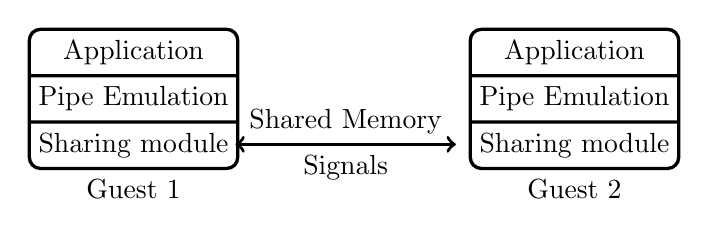
\begin{tikzpicture}
      [domU/.style={
           rectangle split,
           rectangle split parts=3,
           rounded corners,
           draw=black, very thick,
           text centered,
           anchor=three
         },
       ]
    \node [domU, label=below:Guest 1] (dom1) at (-2.8,0) {
      Application
      \nodepart{two}
      Pipe Emulation
      \nodepart{three}
      Sharing module
    };
    
    \node [domU, label=below:Guest 2] (dom2) at (2.8,0) {
      Application
      \nodepart{two}
      Pipe Emulation
      \nodepart{three}
      Sharing module
    };

    \path (-0.3,0.1) edge [draw=black, very thick, <->] node [above] {Shared Memory} node [below] {Signals} (2.5,0.1);
    
  \end{tikzpicture}
  \caption{Optimised channel using shared memory and signals}
  \label{xen_shm}
\end{figure}


Our implementation is divided into two parts. First, the Xen shared memory tool, a device kernel module, provides a way of sharing memory between two user-spaces of possibly different virtual machines on the same Xen hypervisor. For performances purposes and because of possible dead-locks, it also uses a bidirectional event channel and therefore provides the user \emph{wait} and \emph{notify} operations.

The second layer of our solution, a user space library on top of the kernel shared memory module, provides a \emph{file-like} interface, allowing the user to set-up a unidirectional channel and use it to send or receive data. It abstracts the inner work that transforms memory into an optimized circular buffer that only makes necessary system calls.

In the second and third parts of this report, we detail the functioning of those two different elements. And we present, in the fourth part, the performances of our solution. 

\section{Shared memory device}

The first realisation of our project is a Linux kernel module which defines a new device driver. According to the end-to-end principle, it's a really dumb module that just gives the user tools to share memory and signals, without any practical protocol for how to use it. As the Linux kernel, and more precisely its Xen parts, always change, our module is only guaranteed to work on Linux kernel version 3.2.32 (Debian testing), 3.4.9 and 3.5.4 (Gentoo Linux stable).

\subsection{Xen shared memory}

In the normal Xen model, each virtual host have its own memory address space which are mapped to non-overlapping physical memory, providing the usual abstraction of total ownership of the memory space to each host. Nevertheless, the Xen hypervisor can also remap the memory of an host into the address space of another host. In order to do so, an host $A$ must ask the hypervisor to grant the right to use a given part of its physical memory to a given host $B$. The hypervisor will issue a ticket which can be used by the $A$ to map the physical memory from $A$ into its own address space.

The implementation of this protocol can be considered as a potential security breach: from our experiments, we tend to believe that the entropy of the domain id (16 bits) and the ticket (32 bits) is really small (and the tickets seems to be simply increasing). Thus an attacker that obtained access to one of the two hosts, as long as it have access to the userspace tools to map the memory, could also, by guessing or brute-forcing those ids, map the same physical memory and thus spy or modify the data. Such a security problem doesn't come from our system but from Xen, thus we believe that it will be fixed in the near future.

Another restriction of this model concerns hot migration of hosts. If a group of hosts shares two-by-two some memory then none of them can be migrated to another machine as it is not possible to share physical memory between two distant nodes (at least with the current technology). The current sharing mechanism and grant system doesn't provide a way to detect and prevent or cope with such migrations, thus our system will probably utterly crash if this occurs. If thus API are provided by Xen in the future, mechanisms that disable the channel could be implemented.

\subsection{Create shared memory}

In order to share some memory, the memory first needs to be allocated in one of the two hosts, that we will call the \emph{offerer}\footnote{This will have implications for the clean termination and memory freeing, as explained later, see section \ref{Termination}.}. When an host do so, it allocates different things, some pages in the real\footnote{In that case, what he believes real, which is protected by Xen.} physical memory and some address space that will be mapped to it. As grants are given on an host to host basis, the \emph{offerer} needs to know the domain id of the other host which will be called the \emph{receiver}. The exact specification of such exchanges of information, using standard communication paths, is outside the scope of our project\footnote{Reader are invited to look at the simple protocol using UDP that we created for that purpose during our test}. Then, by using an \emph{Hypercall}, the \emph{offerer} can ask the hypervisor to grant the right to map. The hypervisor will store the pseudo-physical address that correspond to the grant, together with the domain id of both the \emph{offerer} and the \emph{receiver} and also a ticket number.

With both the \emph{offerer's} domain id and the grant ticket number, the \emph{receiver} can make another \emph{Hypercall} with some references of its own address space: the hypervisor will take care of modifying the memory mapping between the two spaces. Mapping in the kernel space is easy, as we fully control what happens. Mapping in the user space, a separate domain with a lot of automatic events, is harder as we will explain in the next section.

In fact, we are not using directly the Hypercalls. Those are pretty stable but needs work to be done around them depending on the hardware, the kernel/Xen versions and so on. Recent Linux kernels provide an API to abstract all of this, but this API have recurrent small changes\footnote{For example the function \emph{gnttab\_unmap\_refs} is different between the three kernel we used.} as more functionalities are added. Even if this API is currently more volatile, we still believe that using it will provide a better long-term stability.

\subsection{Map memory into user-space}
\label{userspace}
As this implementation tries to limit the kernel involvement, it maps directly the shared memory into the userspace, allowing direct read/write accesses without any overhead.

On the \emph{offerer} side, the mapping is easy as the kernel already prepare all the work for device drivers: when standard device driver functions are called (open, nmap, munmap, close), the kernel automatically prepare or clean memory needed. Furthermore, a function, \emph{remap\_pfn\_range}, exists for simple remapping, making this remapping a child problem.

On the other side, the \emph{receiver} one, things are more complicated. At first sight, one can simply call the xen API with the user space address. It will somehow work, that is it will map the physical memory and grant the access as we want, but it won't last long as it will taint the kernel with page errors on the unmapping. The correct approach is to work on a lower lever, page tables, and to correctly invalidate the mapping on a early stage of the memory unmapping\footnote{Dedicated MMU Notifier Operation are registered in the memory management system in order to do so.}. This part of our work is inspired by the Linux \emph{gntdev} that allows to map memory into user space (But without all the automatic exchanges nor the signals that we wanted). Even if our code was fully rewritten for simplicity purposes, maintainers and users are encouraged to monitor modifications of this part of the Kernel on each major update as it will be probably be maintained by Linux kernel or Xen developers as new functionalities kicks in.


\subsection{Event channel}



\subsection{Termination}
\label{Termination}

Outside the correct memory invalidation that we talked about in section \ref{userspace}, because of the non-symmetrical model of the memory sharing, special care is needed before completely cleaning the module. The initial physical space belongs to the \emph{offerer}, that internally allocated it, mapped it and told Xen about its exact location. When closing the module, the \emph{offerer} needs to free it as we don't want such enormous memory leakages. But as we are talking about direct mapping, if the \emph{receiver} still have an active mapping, it will be able to modify the physical memory. If the \emph{offerer} frees the memory without any check, it will be potentially re-allocated later somewhere else by any application or kernel actions and if the \emph{receiver} modify it at this point, unspecified errors are expected from the resulting non-desired sharing.

The Xen API provides methods to detect the number of active mappings per grant. As a result our implementation checks for potential active mapping and prevent memory freeing if necessary. From the user point of view, the mapping will be undone and the function call returns immediately but internally information about memory is kept and the unmapping is scheduled to take place later.

\section{Shared memory based circular buffer}

\subsection{Principles}



\subsection{Optimizations}



\subsection{Closure and dead-lock avoidance}






\section{Evaluation}

Because of the instability of the Xen system and of the Linux kernel, it is currently not possible to do an exact comparison between other similar idea/implementation. In order to be as fair as possible we chose to use old hardware that dates from approximately the same period as the quoted related work.

\subsection{Configuration}

Our experiments were run on an Intel\textregistered ~Core\texttrademark 2 Quad Processor Q9550, running at 2.83 GHz with a L2 cache of 12MB and equipped with 4GB of standard DDR2-800 RAM. We are aware that such a system is not representative of recent dedicated virtualisation servers, but results are still impressive. With the recent improvements of caches, sharing mechanisms inside CPUs and memory access, we believe that our system will present far better results on modern systems. For example, tests run inside a virtualised environment on a two years old Intel\textregistered ~i7 processor showed result close to an order of magnitude better that the ones presented in this report, but fairness with other existing implementation was, in our eyes, more important.

The final tests were run using Xen 4.2.1 on top of Linux 3.5.7. We used the Gentoo Linux distribution for both the dom0 and the domUs. We also pinned the CPUs: dom0 always had 2 CPUs and 2GB of memory. Depending on the tests, either we used two hosts with 1 CPU and 1GB of memory each, either we used only one other host with 2 CPUs and still 1GB of memory. We allocated a lot of memory to each hosts but almost none of it was used by our system that only allocate one shared buffer.

\subsection{Throughput}

\begin{figure}[h]
\centering
\begin{tikzpicture}
    \begin{semilogxaxis}[
        xlabel=Buffer size (KiB),
        ylabel=Throughput (Gbps),
        legend style={nodes=right},
        legend pos= north west,
        scaled ticks=false, 
        compat=1.3
        ]
        
    \addplot table [ x index=0,y index=1] {plots/bandwidth.txt};
    \addlegendentry{Xen pipe}
    
    \addplot table[ x index=0,y index=3] {plots/bandwidth.txt};
    \addlegendentry{Stressed Xen pipe}
    
    \addplot table[ x index=0,y index=2] {plots/bandwidth.txt};
    \addlegendentry{TCP}
    
    
    \end{semilogxaxis}
\end{tikzpicture}
\caption{Comparison between Xen pipe and TCP throughputs for different buffer sizes}
\label{shm_size}
\end{figure}


\begin{figure}[h]
\centering
\begin{tikzpicture}
    \begin{semilogxaxis}[
        xlabel=Message size (Bytes),
        ylabel=Throughput (Gbps),
        legend style={nodes=right},
        legend pos= north west,
        scaled ticks=false, 
        compat=1.3
        ]
        
        
        \addplot table[x index=0,y index=4] {plots/messageSize.txt};
    \addlegendentry{XenPipe: 60}
        
      \addplot table[ x index=0,y index=3] {plots/messageSize.txt};
    \addlegendentry{XenPipe: 20}  
        
        
     \addplot table[  x index=0,y index=2] {plots/messageSize.txt};
    \addlegendentry{XenPipe: 5}   
        
    \addplot table[  x index=0,y index=1] {plots/messageSize.txt};
    \addlegendentry{XenPipe: 1}
    
    
    \addplot [smooth,dashed,mark=*,orange] table[  x index=0,y index=5] {plots/messageSize.txt};
    \addlegendentry{XWay}
    
    \addplot [smooth,dashed,mark=square*, violet]  table[  x index=0,y index=7,orange] {plots/messageSize.txt};
    \addlegendentry{XenSocket}

    \addplot [smooth,dashed,mark=x, magenta] table[  x index=0,y index=6] {plots/messageSize.txt};
    \addlegendentry{XenLoop}
   
    \end{semilogxaxis}
\end{tikzpicture}
\caption{Throughput of Xen Pipe with different shared memory sizes (indicated in pages) and other state-of-the-art solutions with respect to the message size}
\label{msg_size}
\end{figure}


\subsection{Delays}

\subsection{Simultaneous transfers}



\begin{figure}[h]
\centering
\begin{tikzpicture}
    \begin{semilogyaxis}[
        xlabel=Number of parallel flows,
        ylabel=Throughput (Mbps),
        legend style={nodes=right},
        legend pos= south west,
        scaled ticks=false, 
        y tick label style={/pgf/number format/.cd,sci,precision=5},
        compat=1.3,
        ]
        
        
        \addplot [blue,mark=x] table[x index=0,y index=1] {plots/multi.txt};
    \addlegendentry{Total throughput}
        
     
    
    \addplot [smooth, red] table[x index=0,y index=8] {plots/multi.txt};
    \addlegendentry{Optimal sharing}
    
     %\addplot [smooth, black] table[x index=0,y index=5] {multi.txt};
    %\addlegendentry{Median value}
    
    %\addplot [smooth, gray] table[x index=0,y index=6] {multi.txt};
    
    %\addplot [smooth, gray] table[x index=0,y index=7] {multi.txt};
       
    %\addplot [smooth, lightgray] table[x index=0,y index=3] {multi.txt};
    
    %\addplot [smooth, lightgray] table[x index=0,y index=4] {multi.txt};
    
    \addplot [box plot median] table {plots/boxes.txt};
    \addplot [box plot box] table {plots/boxes.txt};
    \addplot [box plot top whisker] table {plots/boxes.txt};
    \addplot [box plot bottom whisker] table {plots/boxes.txt};
    \addlegendentry{Values distribution}

    
    \end{semilogyaxis}
\end{tikzpicture}
\caption{Throughputs of multiple parallel flows (60 shared pages per transfert - messages of 32KiB - average value over more than 20 seconds). The dark line corresponds to the median value. 
Gray lines correspond to first and last decile. Light gray lines correspond to the maximum and minimum values}
\label{simult_flows}
\end{figure}





\section{Conclusion}

\subsection{Contributions}


\subsection{Possible improvements}







 
% if have a single appendix:
%\appendix[Proof of the Zonklar Equations]
% or
%\appendix  % for no appendix heading
% do not use \section anymore after \appendix, only \section*
% is possibly needed

% use appendices with more than one appendix
% then use \section to start each appendix
% you must declare a \section before using any
% \subsection or using \label (\appendices by itself
% starts a section numbered zero.)
%


%\appendices
%\section{Figures}
%Appendix one text goes here.




% you can choose not to have a title for an appendix
% if you want by leaving the argument blank

%Appendix two text goes here.


% use section* for acknowledgement
%\section*{Acknowledgment}
%
%
%The authors would like to thank...



% Can use something like this to put references on a page
% by themselves when using endfloat and the captionsoff option.
\ifCLASSOPTIONcaptionsoff
  \newpage
\fi



\begin{thebibliography}{1}

\bibitem{XenSocket}
Xiaolan Zhang et al., \emph{XenSocket: A High-Throughput Interdomain Transport for Virtual Machines}, Middleware '07.

\bibitem{XWay}
Kangho Kim et al., \emph{Inter-domain Socket Communications Supporting High Performance and Full Binary Compatibility on Xen}, VEE '08.

\bibitem{XenLoop}
Jian Wang et al., \emph{XenLoop : A Transparent High Performance Inter-VM Network Loopback}, HPDC '08.

\bibitem{gntdev}
Derek G. Murray, Grzegorz Milos and Steven Hand, \emph{Improving Xen Security through Disaggregation}, VEE '08.

\end{thebibliography}





% that's all folks
\end{document}


